
\chapter{预等离子体对于加速的增强作用}
\label{chap:preplasmaEhancement}




\section{}
\begin{figure}[!htbp]
  \centering
  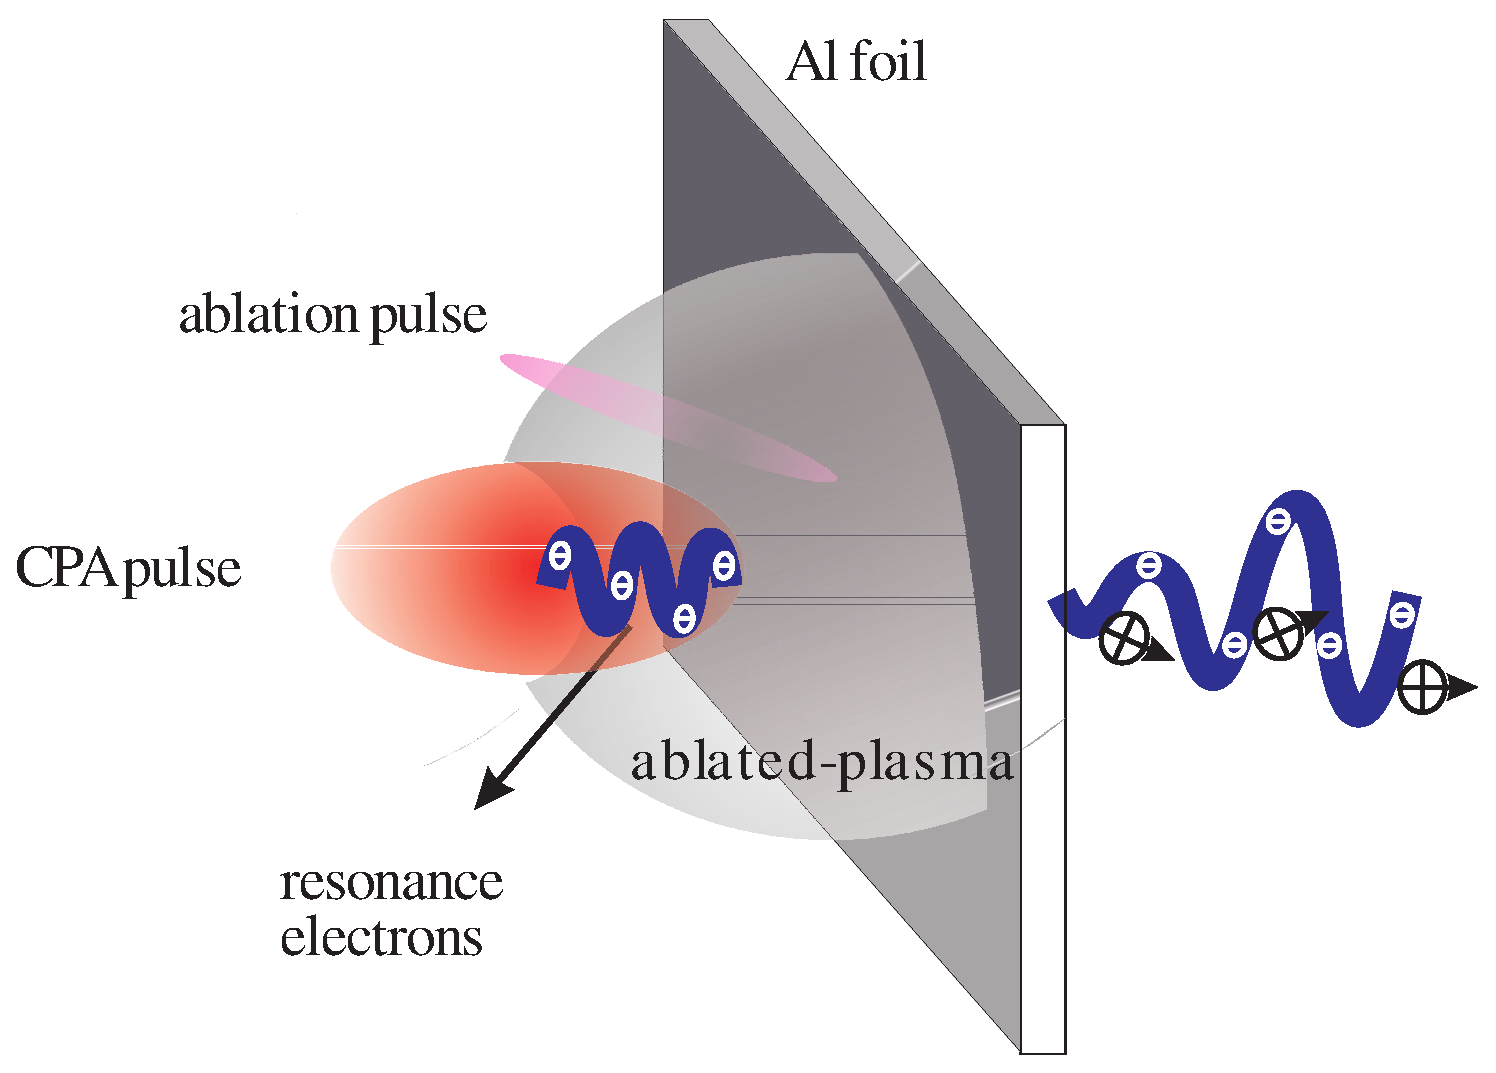
\includegraphics[width=\MyFactor\textwidth]{Img/enhancement.eps}
  \caption{预脉冲增强作用示意图}
  \label{fig:prepulse2012}
\end{figure}

上一章中,我们利用激光的预脉冲或者中等强度激光脉冲($10^{10}W/cm^2$ 到 $10^{14}W/cm^2$),对于金属靶进行烧蚀,产生预等离子体。预等离子体由靶前表面向外传播,其密度一维分布为类指数函数,其中一部分处于临界密度领域。我们已经对于临界密度做出定义,与激光频率一致的等离子体波对应的密度,同时也是非相对论激光脉冲穿透密度极限。当等离子体密度高于临界密度之后,激光无法穿透等离子体,很大一部分能量被反射。由于等离子体中激光的频率${\omega}^2={{\omega}_p}^2/{\gamma} +k^2 c^2$,其中${{\omega}_p}^2=4 {\pi}^2 n_e/m $,当激光的光强到达相对论区域,由于电子质量的增加,因此激光穿透等离子体的能力增强,这种线性被称为相对论自导引穿透。
由于激光可以穿透等离子体,从而使得激光与等离子体作用距离变长。同时由于等离子体中的非线性现象,激光在等离子体中的能量转换效率得到了很大的提高。由于激光脉冲强度在横纵向存在一定分布,一般情况下为高斯分布,因此有质动力在横向上也存在类似的分布,使得横向上电子被排开的程度不同,等离子体的密度分布不再均匀。对应于等离子体的折射率的变化,使得中心处的折射率变小,而两边的折射率较大,类似于透镜的聚焦属性。同时对于相对论激光的径向分布,使得电子的质量的相对论增加也存径向分布,中心处的电子的质量偏大,而两翼出的电子的质量相对较小,影响等离子体的折射率。这种由激光脉冲对于等离子体折射率的调制,改变激光在传播过程中的聚焦属性的现象称为相对论自聚焦。另一方面,由于激光存在纵向的分布,假设纵向分布为高斯分布,激光的光强对于激光脉冲包络各部分的群速度产生调制作用,包络峰值处的光强较高,群速度快于其他部分,使得脉冲整体上呈现在线前移动,脉冲前沿变得陡峭,这种效应称为相对论自调制。

\begin{figure}[!htbp]
  \centering
  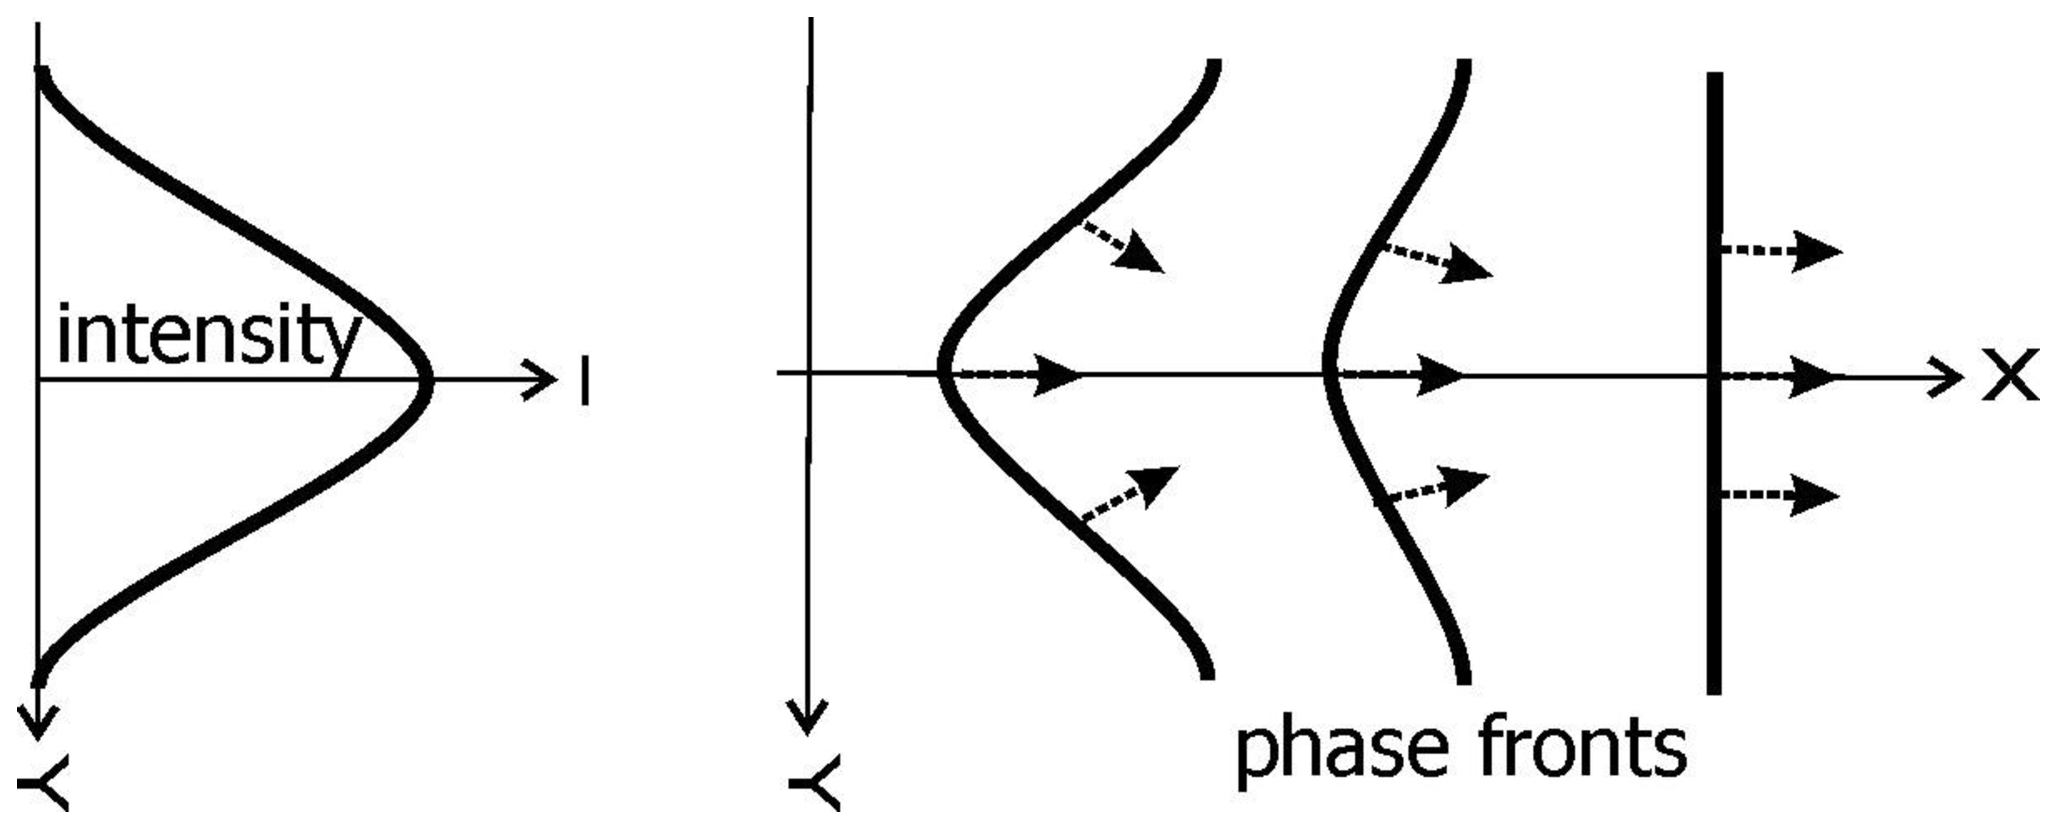
\includegraphics[width=\MyFactor\textwidth]{Img/selffocussing.eps}
  \caption{激光自聚焦示意图}
  \label{fig:selffousing}
\end{figure}

\begin{figure}[!htbp]
  \centering
  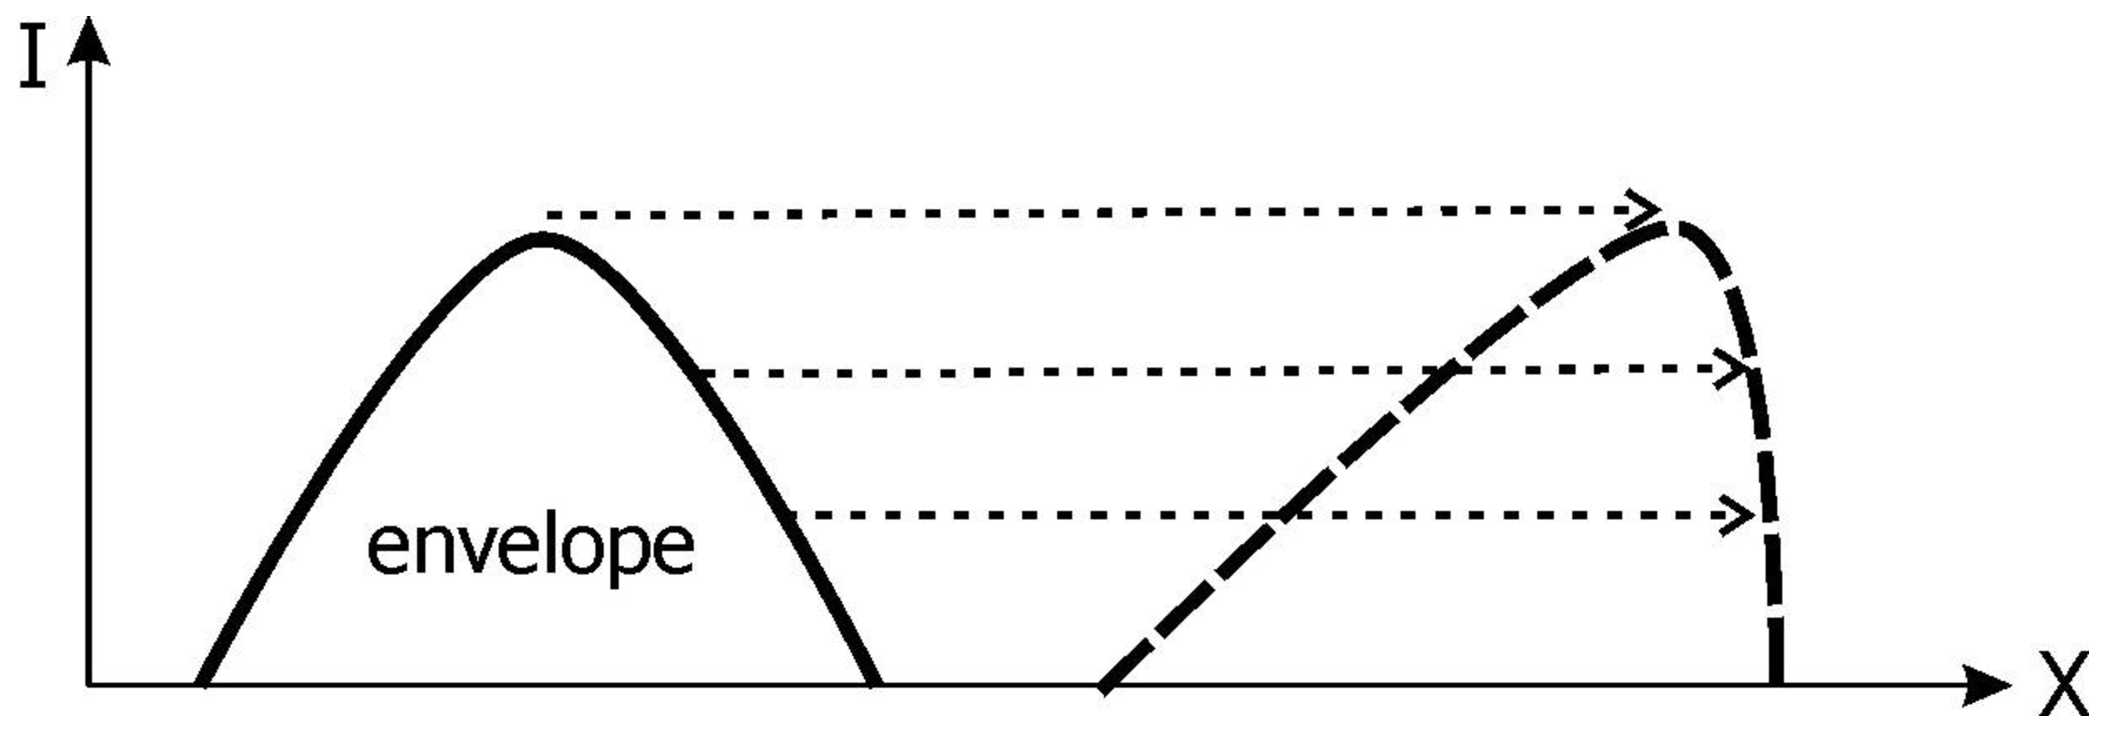
\includegraphics[width=\MyFactor\textwidth]{Img/prof-steepening.eps}
  \caption{激光自相位调制}
  \label{fig:phaseModulate}
\end{figure}

由于激光在临界密度等离子体中传播时,能量转换效率 得到了很大的提高,在激光与等离子体相互作用中有着广泛的应用。



 相对论自聚焦透镜\cite{wang2011laser},是相对论强度激光在临界密度等离子体中传播,当激光光强与等离子体密度匹配时,由自聚焦与自调制共同作用。使得激光在横向上焦斑变小,纵向上脉冲尺寸压缩。光强得到一个数量级的提高,同时激光的对比度明显地提高。


自匹配共振电子加速,研究了相对论激光在等离子体的传播过程中,当激光的强度与等离子体的密度存在一定的匹配关系时,电子在通道中得到捕获,并能够与激光的电场发生强烈的共振的现象的。而这种匹配关系对应的电子在通道中的运动得到了细致的描述。这种电子具有能量高且在时间以及空间上具有很强的谐振性,可用于高频率高品质的辐射的研究,是$\gamma$光源的重要途径。 Nakamura等人通过模拟发现,当激光在变化密度的临界密度等离子体中的传播时。激光可以穿透等离子体,并在其中稳定的传播,而当等离子体的密度发生突然变化的时候,在密度变化区域,一种磁场涡旋出现。这种磁涡旋结构的特点,纵向产生有效的加速电场,在横向产生对于离子的聚焦效应对于电子的散焦的效应。处于涡旋内部的质子被此结构捕获并得到能量增益,并且自在纵向存在聚焦的效果。最终,可以实现准准单能且高聚焦的离子束流。在理论研究取得重要进步的同时,在实验中也有很多优秀的工作,Mcknenna等人在实验上实现了预等离子体对于加速的增强效应。实验中使用中的强度烧蚀脉冲对于金属靶表面进行烧蚀的方法制备临界密度等离子体,其中与脉冲的持续时间可以控制,从而得到不同的预等离子体的分布。在进行了不同预脉冲尺寸的实验后,最终得到了最高能量38$MeV$的质子束流,相对于没有预脉冲的情况产生$25 \%$的能量提高。然而此实验中很多的情况是可以优化的,而这一问题在后续将讨论。同时在临界密度等离子体的制备领域同样产生很重要的进步,Zoni等人2013年在实验上,利用间歇式脉冲激光实现了准均匀密度的泡沫等离子体的制备,其等离子体的密度以及厚度都可以得到有效的控制。2014年Passoni等人基于这种等离子体进行了质子加速的实验,使用非相对论强度的激光,使得最终的离子能量提高达到3倍之多。诸多的理论和实验工作都预示这这一领域中巨大的潜力。



\section{预脉冲与预等离子体}



在相对论自聚焦的过程中,激光脉冲在等离子体中传播,激光波前位置的电子被激光有质动力排开,通道中的离子由于质量惯性较大,最终形成横向尺寸与激光焦斑大小,离子背景的通道结构。通道中电子密度中间低,两侧较高,且通道壁的电子由于回流效应产生轴向磁场。同时在离子背景通道中,由于电子与离子在通道中静电分离,通道中形成了的静电势。
通道中的电子在轴向磁场以及静电场的共同作用下,产生betatron震荡。此外,这些betatron共振电子受到激光场的驱动作用,当betatron震荡频率与激光频率匹配时,共振现象发生,使得电子产生强烈的能量吸收,这种现象被称为DLA(Direct Laser Acceleration)。共振电子的横向动量由于共振效应得到了很大的增益, 其横向震荡频率即激光频率$\omega_0$。同时在磁场的作用下,一部分的横向能量转化为纵向的能量, 且$v_{\parallel} = 1- {v_{\perp}}^2$,纵向的频率是$2 \omega_0$。
\begin{figure}[!htbp]
  \centering
  \includegraphics[width=\MyFactor\textwidth]{Img/DLAmomentum.eps}
  \caption{DLAeMomentum}
  \label{fig:selffousing}
\end{figure}

由于强磁场的存在,DLA电子在通道中紧聚焦,高能量密度电子束流沿激光传播方向运动。关于DLA的系统研究属于A. Pukhov和J. Meyer-ter-Vehn以及盛正明\cite{pukhov1998relativistic,pukhov1999particle},通过模拟和实验,得出电子的温度的定标率,
\begin{equation}
\label{eqn:DLAtemperature}
T_e = 1.8(I_{cpa} {\lambda}^2/{13.7}GW)^{1/2}
\end{equation} 



由于这种加速过程中,电子的运动类似自由电子激光中的wiggler,因此这种加速也被称为逆自由电子激光电子加速。其电子加热温度相对于传统的有质动力加速过程的电子温度, 有将近三倍以上的提高,而且由于通道中磁场的聚焦效果,因此电子束流的密度较高。
\begin{figure}[!htbp]
  \centering
  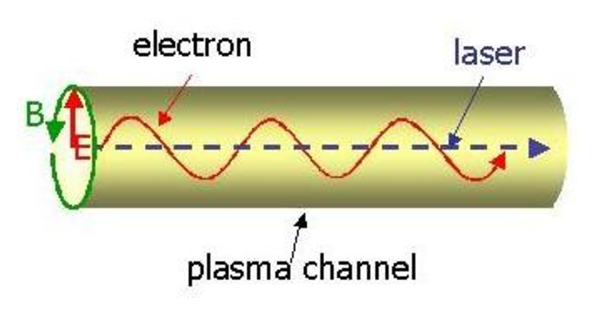
\includegraphics[width=\MyFactor\textwidth]{Img/IFEL.eps}
  \caption{逆自由电子激光示意图}
  \label{fig:IFEL}
\end{figure}









理论和实验工作中已经有很多的结果与共振电子有关,王鸿勇等人\cite{wang2011high}在2011年的理论工作提到,使用均匀临界密度的等离子体以及薄膜靶,可以实现3倍左右的能量提高,同时束流品质得到相应的提高。Sgattoni等人\cite{sgattoni2012laser}在2012通过二维以及三维的模拟细致地研究了激光在等离子体中的聚焦以及后续的加速的过程,最终也得到了质子能量明显增加的结论。实验中有上文提到的 macknna 在2008年所完成的实验,以及
Glinec等人\cite{glinec2008evolution}在2008年完成的实验,实验中使用预脉冲对于靶进行烧蚀,而后使用主激光进行离子加速。实验结果表明,一部分的烧蚀作用对于加速的作用是增强的,而另一部分起到负面的作用。在以上的工作中, 将临界密度等离子体对于离子加速的增强效应的原因归结为:1 激光脉冲在等离子体中的聚焦,使得激光的光强得到提高;2 高能电子的产生以及激光自聚焦的共同作用的结果。然而这种增强效果的根本原因是什么,在已有激光设备的基础上如何获得最优的质子加速效果,以及这种加速的实际的潜力有多少,这些问题都是需要更多的工作来澄清的。

本文中,延续了实验中采烧蚀脉冲作用于靶前表面产生预等离子体的方法,研究预脉冲产生的预等离子体对于加速的增强效应。强度$10^{12}-10^{14} W/cm^2$,脉冲时间$100ps$量级烧蚀脉冲与
$\mu m$量级的金属靶作用,烧蚀激光脉冲对于靶前表面离化加热,使得前表面的等离子体膨胀。通过调整烧蚀脉冲的强度以及持续时间,控制金属靶的烧蚀深度和预等离子体膨胀距离以及密度分布梯度,最终未烧蚀的靶和膨胀的等离子体形成了气体与固体薄膜靶的双层靶结构。当主激光到来的时候,先于气体作用,自聚焦的同时,产生高能高密度的DLA共振电子。
激光能量有效地转化给电子,而后电子传播至靶后形成鞘层场加速离子,最终对于离子加速产生增强的作用。
激光的自聚焦不是加速增强效应的主要原因,高能高密度DLA电子是真正的增强效应的主体。
共振电子的温度$T_e=1.8(I_{cpa}{\lambda}^2/{13.7}GW)^{1/2}$\cite{pukhov1999particle},
相对于有质动力加热电子温度$T_e=0.5[(1+(I_{cpa}{\lambda}^2/{13.8}GW)/2)^{1/2}-1]$\cite{wilks1992absorption},有三倍以上的提高。同时高密度高能DLA电子经过薄膜靶,在其后表面形成鞘层场,强度$E_{sheath}= (\frac{8 \pi}{e_N} n_e T_e)^{1/2}$ \cite{mora2003plasma}, $e_N \approx 2.71828$是欧拉常数。鞘层加速中的质子最高能量$E_{max} \propto T_e[In(2\tau)]^2$,其中 $\tau \propto \sqrt{n_e} \tau_{laser}$,$\tau_{laser}$是激光的脉冲持续时间。由加速电场以及最高能量的公式可知,电子的温度以及密度对于加速都是由作用的。提高电子的温度,需要把激光能量尽可能多的传递给电子,这一点在DLA加热中完成。同时通道的存在使得DLA电子聚焦在通道,保证了电子的密度。确保激光能量尽量多传递,同时满足电子一直处于通道聚焦,就可以实现最优的加速。因此最优的加速条件:
激光在即将达到固体靶的时候耗尽所有的能量,即DLA共振电子获得最大程度的能量增益的同时,确保激光脉冲产生的通道能够一直连接到金属靶,有助于电子保持聚焦的高密度状态。如果预等离子体的膨胀尺寸不够,电子得不到足够的激光能量转换,温度较低。相反,如果预等离子体的膨胀尺寸过长,激光会在预等离子体中耗散,但在激光吸收完全之后,通道随之消失,无法将高能量高密度DLA电子传输到未烧蚀靶。综合考虑共振电子的产生和传输过程,很大程度上决定于预等离子体的密度,因此可以通过控制预脉冲的参数,得到最优条件。对于最优条件下的加速,我们有如下的估计:




1激光的焦斑半径$r_0$与通道半径相当
2激光能量有到共振电子的比例为$\alpha$, 于是共振电子能量$E_{e} =\alpha E_{laser} $,且$E_{laser}=\pi {w_0}^2 I_{cpa} \tau_{cpa}$
3当共振电子的温度最高时,其能量可估计为:

\begin{equation}
\label{eqn:energyOsilationElectron}
 \pi {w_0}^2 {{\int}_{0}}^{x_{front}} density(x) \times T_e
\end{equation}

其中 $x_{front}=c_s {\tau}_{abl}[2ln({\tau}_{abl} {\omega}_{pi})+ln2-3]$\cite{mora2003plasma}    是预等离子体膨胀前沿,预等离子体密度分布$density(x)=n_c exp(-x/{c_s{\tau}_{abl}})$, ${\omega}_{pi}$是热电子对应等离子体频率, ${\tau}_{abl}$是烧蚀脉冲时间尺寸,烧蚀脉冲强度$I_{abl}$ 包括在离子声速$c_s$中。考虑条件2,得到



\begin{equation}
\label{eqn:OptimalCondition}
{1.8} c_s {\tau}_{abl}[1-exp(-x_{front}/{c_s{\tau}_{abl}})] 
 = {\alpha}_{absorb} a_{cpa} \tau_{cpa}.
\end{equation}







在此理论分析基础上我们做了模拟仿真的研究,二维PIC粒子仿真,使用KLAP代码,参数依据北京大学强激光实验室条件,金属靶材质是密度为2.7$g/cm^3$铝靶,厚度为$\mu m$量级。激光参数包括有:预脉冲以及主脉冲。预脉冲的强度: $10^12W/cm^2$,且预脉冲的时间尺度为1ns之内。主激光脉冲在预脉冲之后,脉冲能量为5J,激光的脉冲持续时间为$30fs$,聚焦后的焦斑半径为5$\mu m$,相应强度$10^20W/cm^2$。靶结构为双层靶,10$\mu  m$量级的预等离子体与$\mu m$厚度的金属靶,其密度分布以及温度电离态等,由MULTI计算的结果导入。 PIC模拟中的参数如下:仿真区域$80 \times 40 \mu m^2$,格点数目$6400 \times 3200$, 其分辨率为$\lambda / 80$。仿真时间为200T, $T=3.3fs$为激光周期。通过改变预脉冲的持续时间,得到不同的密度分布,得出了三组仿真结果。



对于仿真的结果我们的分析如下:
首先分析出射质子能量最高组。激光在预等离子体中传播并将能量传递给共振电子的过程。如图所示(\ref{fig:laserEvolution}),在其中\ref{fig:laserEvolution}(a) 是激光聚焦的过程,$t=50T$的时候激光开始进入预等离子体,并在其中传播。之后$t=80$脉冲进入强聚焦的过程,激光的强度的增加剧烈,并且伴随着不稳定性的出现。$t=100T$激光波前达到金属靶的位置,其能量基本耗散。整个过程中,激光的能量很少有反射的成分,伴随着聚焦过程的增强,共振电子产生。在\ref{fig:laserEvolution}(b),电子的能量密度分布。 其中心位置处的电子呈现出明显的周期性结果,且其周期为激光的周期,而不是由于所谓的有质动力加速所产生的二倍于激光频率的结构。与此同时,紧聚焦的电子束流达到靶后,形成鞘层场,促进加速作用。在\ref{fig:laserEvolution}(c)显示了,激光脉冲耗散完之后离子通道的分布,其连接于靶前表面处,有效的保证了共振电子的束流品质。


\begin{figure}[!htbp]
  \centering
  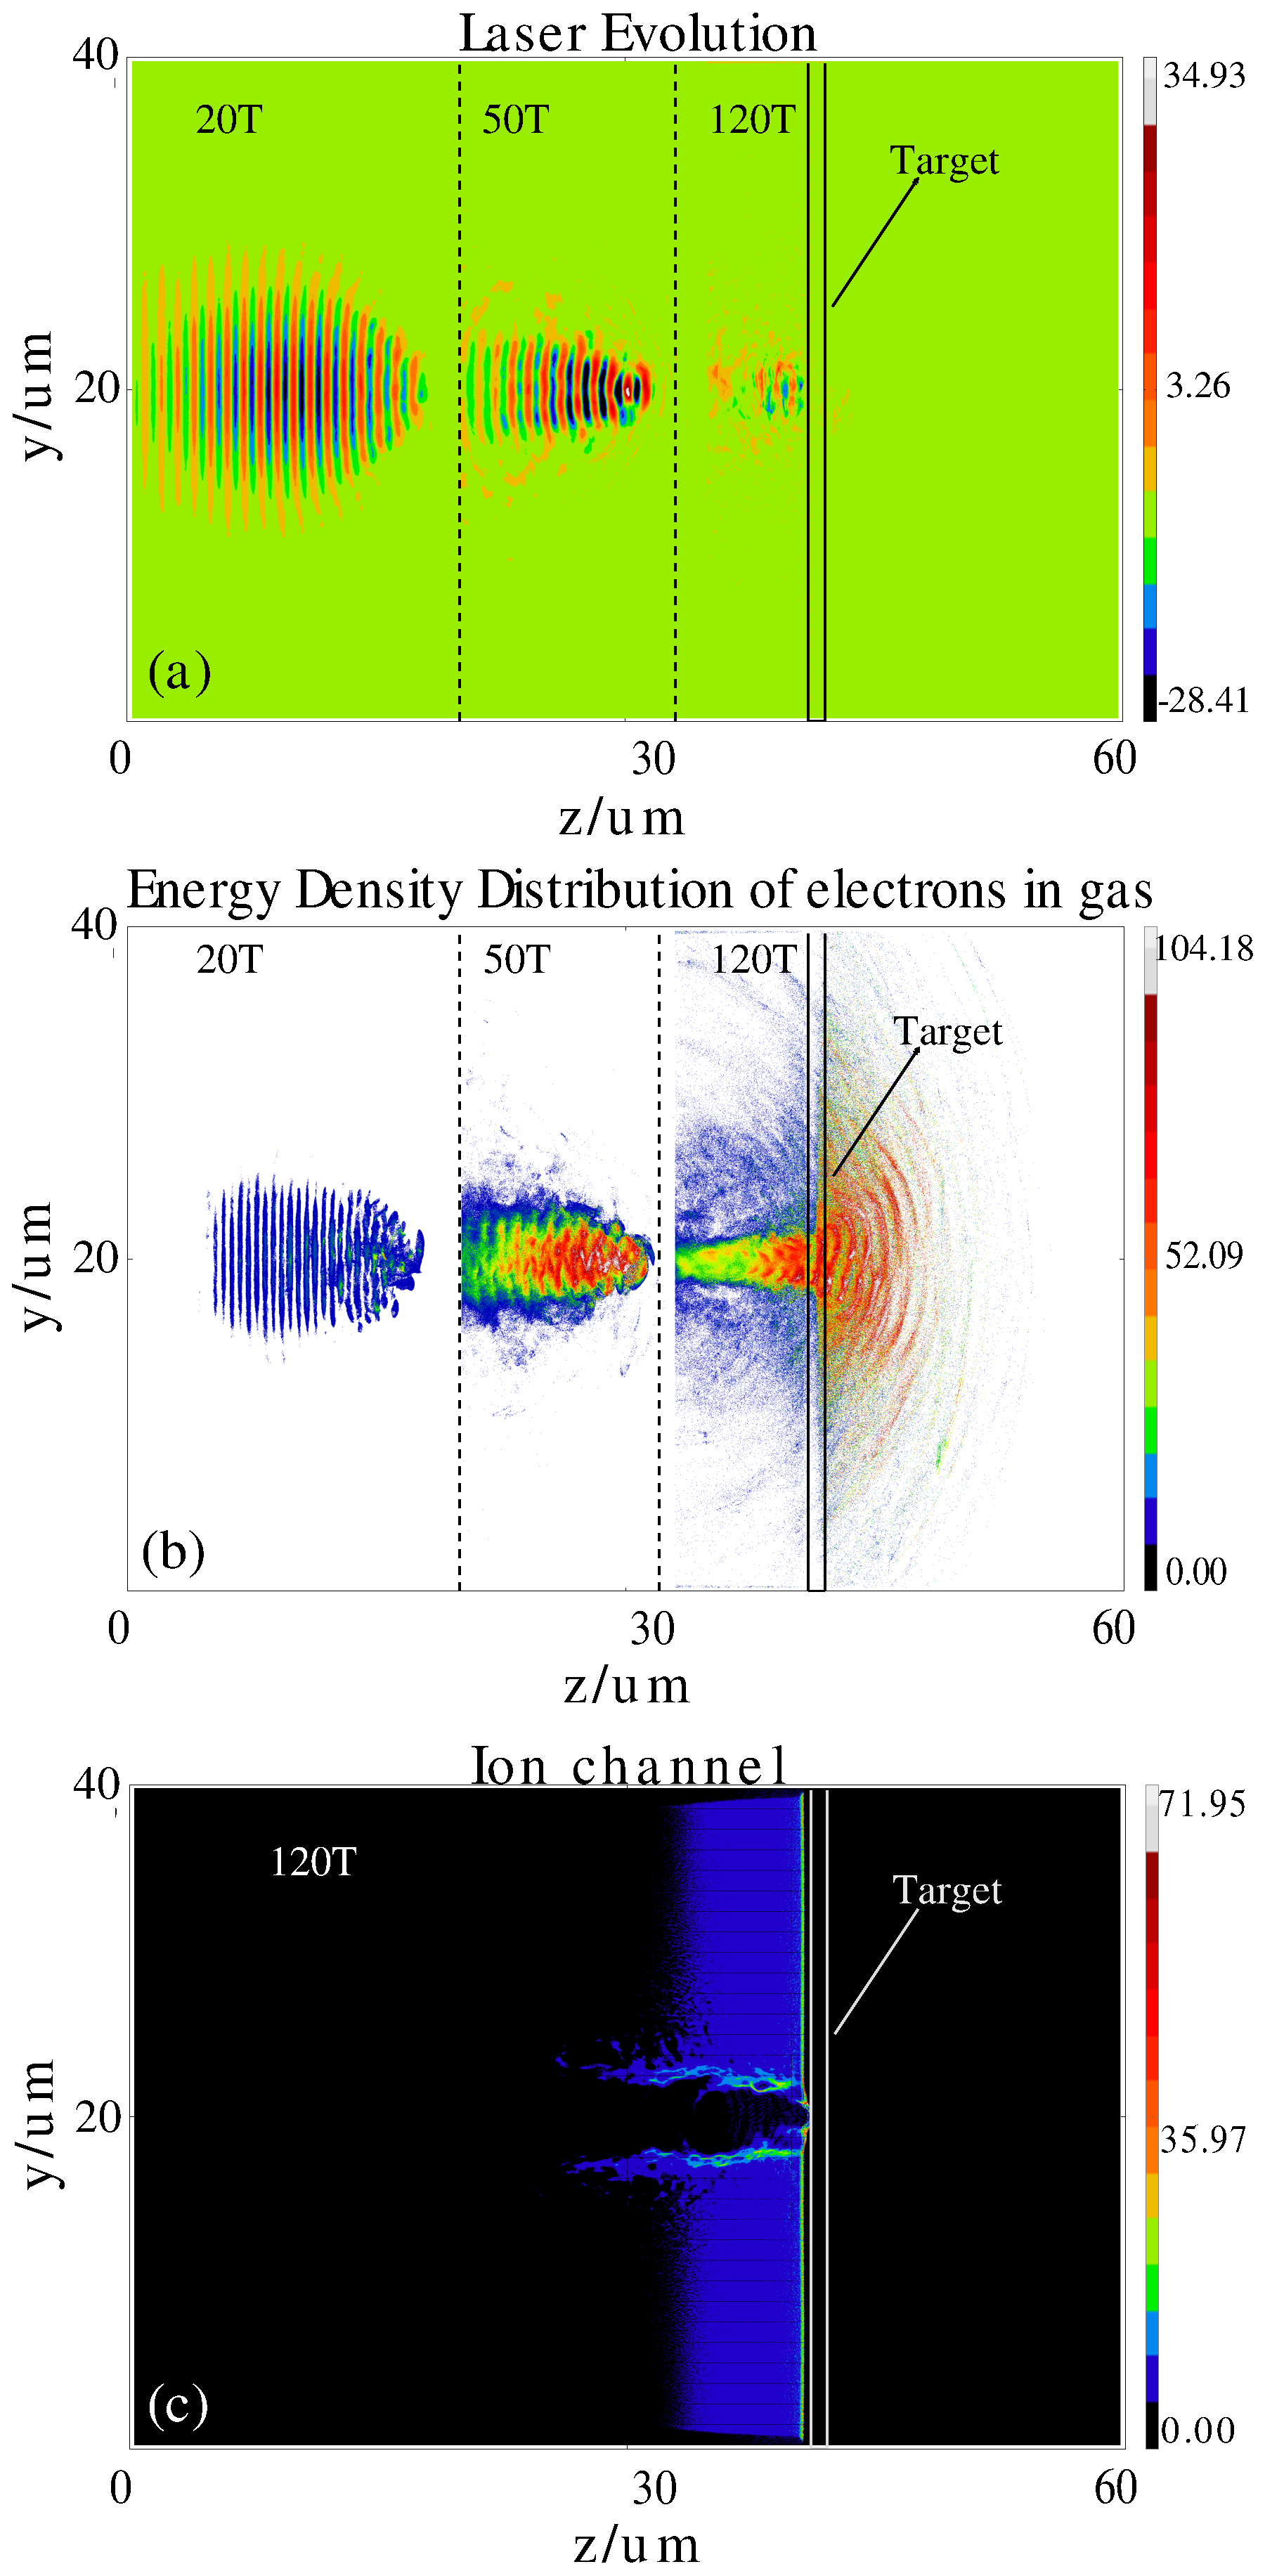
\includegraphics[width=\MyFactor\textwidth]{Img/laserEvolution.eps}
  \caption{激光聚焦及共振电子产生和传输}
  \label{fig:laserEvolution}
\end{figure}


另外两组能量较低的仿真结果在 \ref{fig:laserEvolution1} 中,其中一组,烧蚀脉冲的持续时间为100ps,称为‘短脉冲’,另一组的烧蚀脉冲持续时间为280ps,称为‘长脉冲’。不同的脉冲长度,对应的结果就是预等离子体密度分布的变化,其中‘短脉冲’对应的膨胀距离较小,而且等离子体的密度中梯度较大。而‘长脉冲’对应的等离子体的膨胀距离较大,而且密度梯度较小。同样做了激光脉冲聚焦在\ref{fig:laserEvolution1}(a)中, 左侧‘短脉冲’组中,激光在没有达到最优聚焦的时候已经被反射了,而右侧的激光脉冲在没有达到固体靶的时候已经完全的耗散,很显然,激光在‘长脉冲’组里的吸收更充分。对应于共振电子的产生的情况在\ref{fig:laserEvolution1}(b),其中‘短脉冲’中电子的能量密度较低原因在于激光能量未能完全的转化,右侧‘长脉冲’电子能量密度在 激光聚焦区域相对较高高。但是, 在‘长脉冲’中,由于激光在耗散之后,通道也就随之消失,没有相应的通道提供聚焦磁场,因此电子很快就散开。\ref{fig:laserEvolution1}(c)中给出了通道的形成,‘长脉冲’中,激光脉冲无法完全穿透预等离子体,从而无法实现通道连接到固体靶。 为了更好地理解等离子体中的电子的加热的情况,我们将电子的加热分区域进行了统计,包括:预等离子体中的电子以及固体靶中的电子。ref{fig:laserAbsorption}(b)为预等离子体中的电子加热的情况,其中红,黑,蓝分别代表着‘最优’,‘短脉冲’,‘长脉冲’的等离子体分布。‘最优’和‘长脉冲’的预等离子体中的电子加热情况类似,可见都已经达到了共振电子加热的极限的情况,而‘短脉冲’中的电子加热由于激光的吸收不完全,能量较低。在ref{fig:laserAbsorption}(c),统计了固体靶中的电子的能谱,‘最优’,‘长脉冲’情况中由于激光在达到靶的时候已经基本耗散,所有没有太多的能量沉积在固体靶子中,而对于‘较短’,电子的加热很明显,由于激光脉冲在固体靶表面有很强烈的反射,因此加热存在。考虑电子的平均温度以及数目,‘长脉冲’,‘最优’相对于‘较短’有着明显的优势,但是由于‘长脉冲’情况下,通道随于激光耗尽而消失,因此无法进一步进行共振电子的聚焦,造成了ref{fig:laserEvolution1}(d)所示的束流散开的情况,对于最终的加速有一定的影响。


\begin{figure}[!htbp]
  \centering
  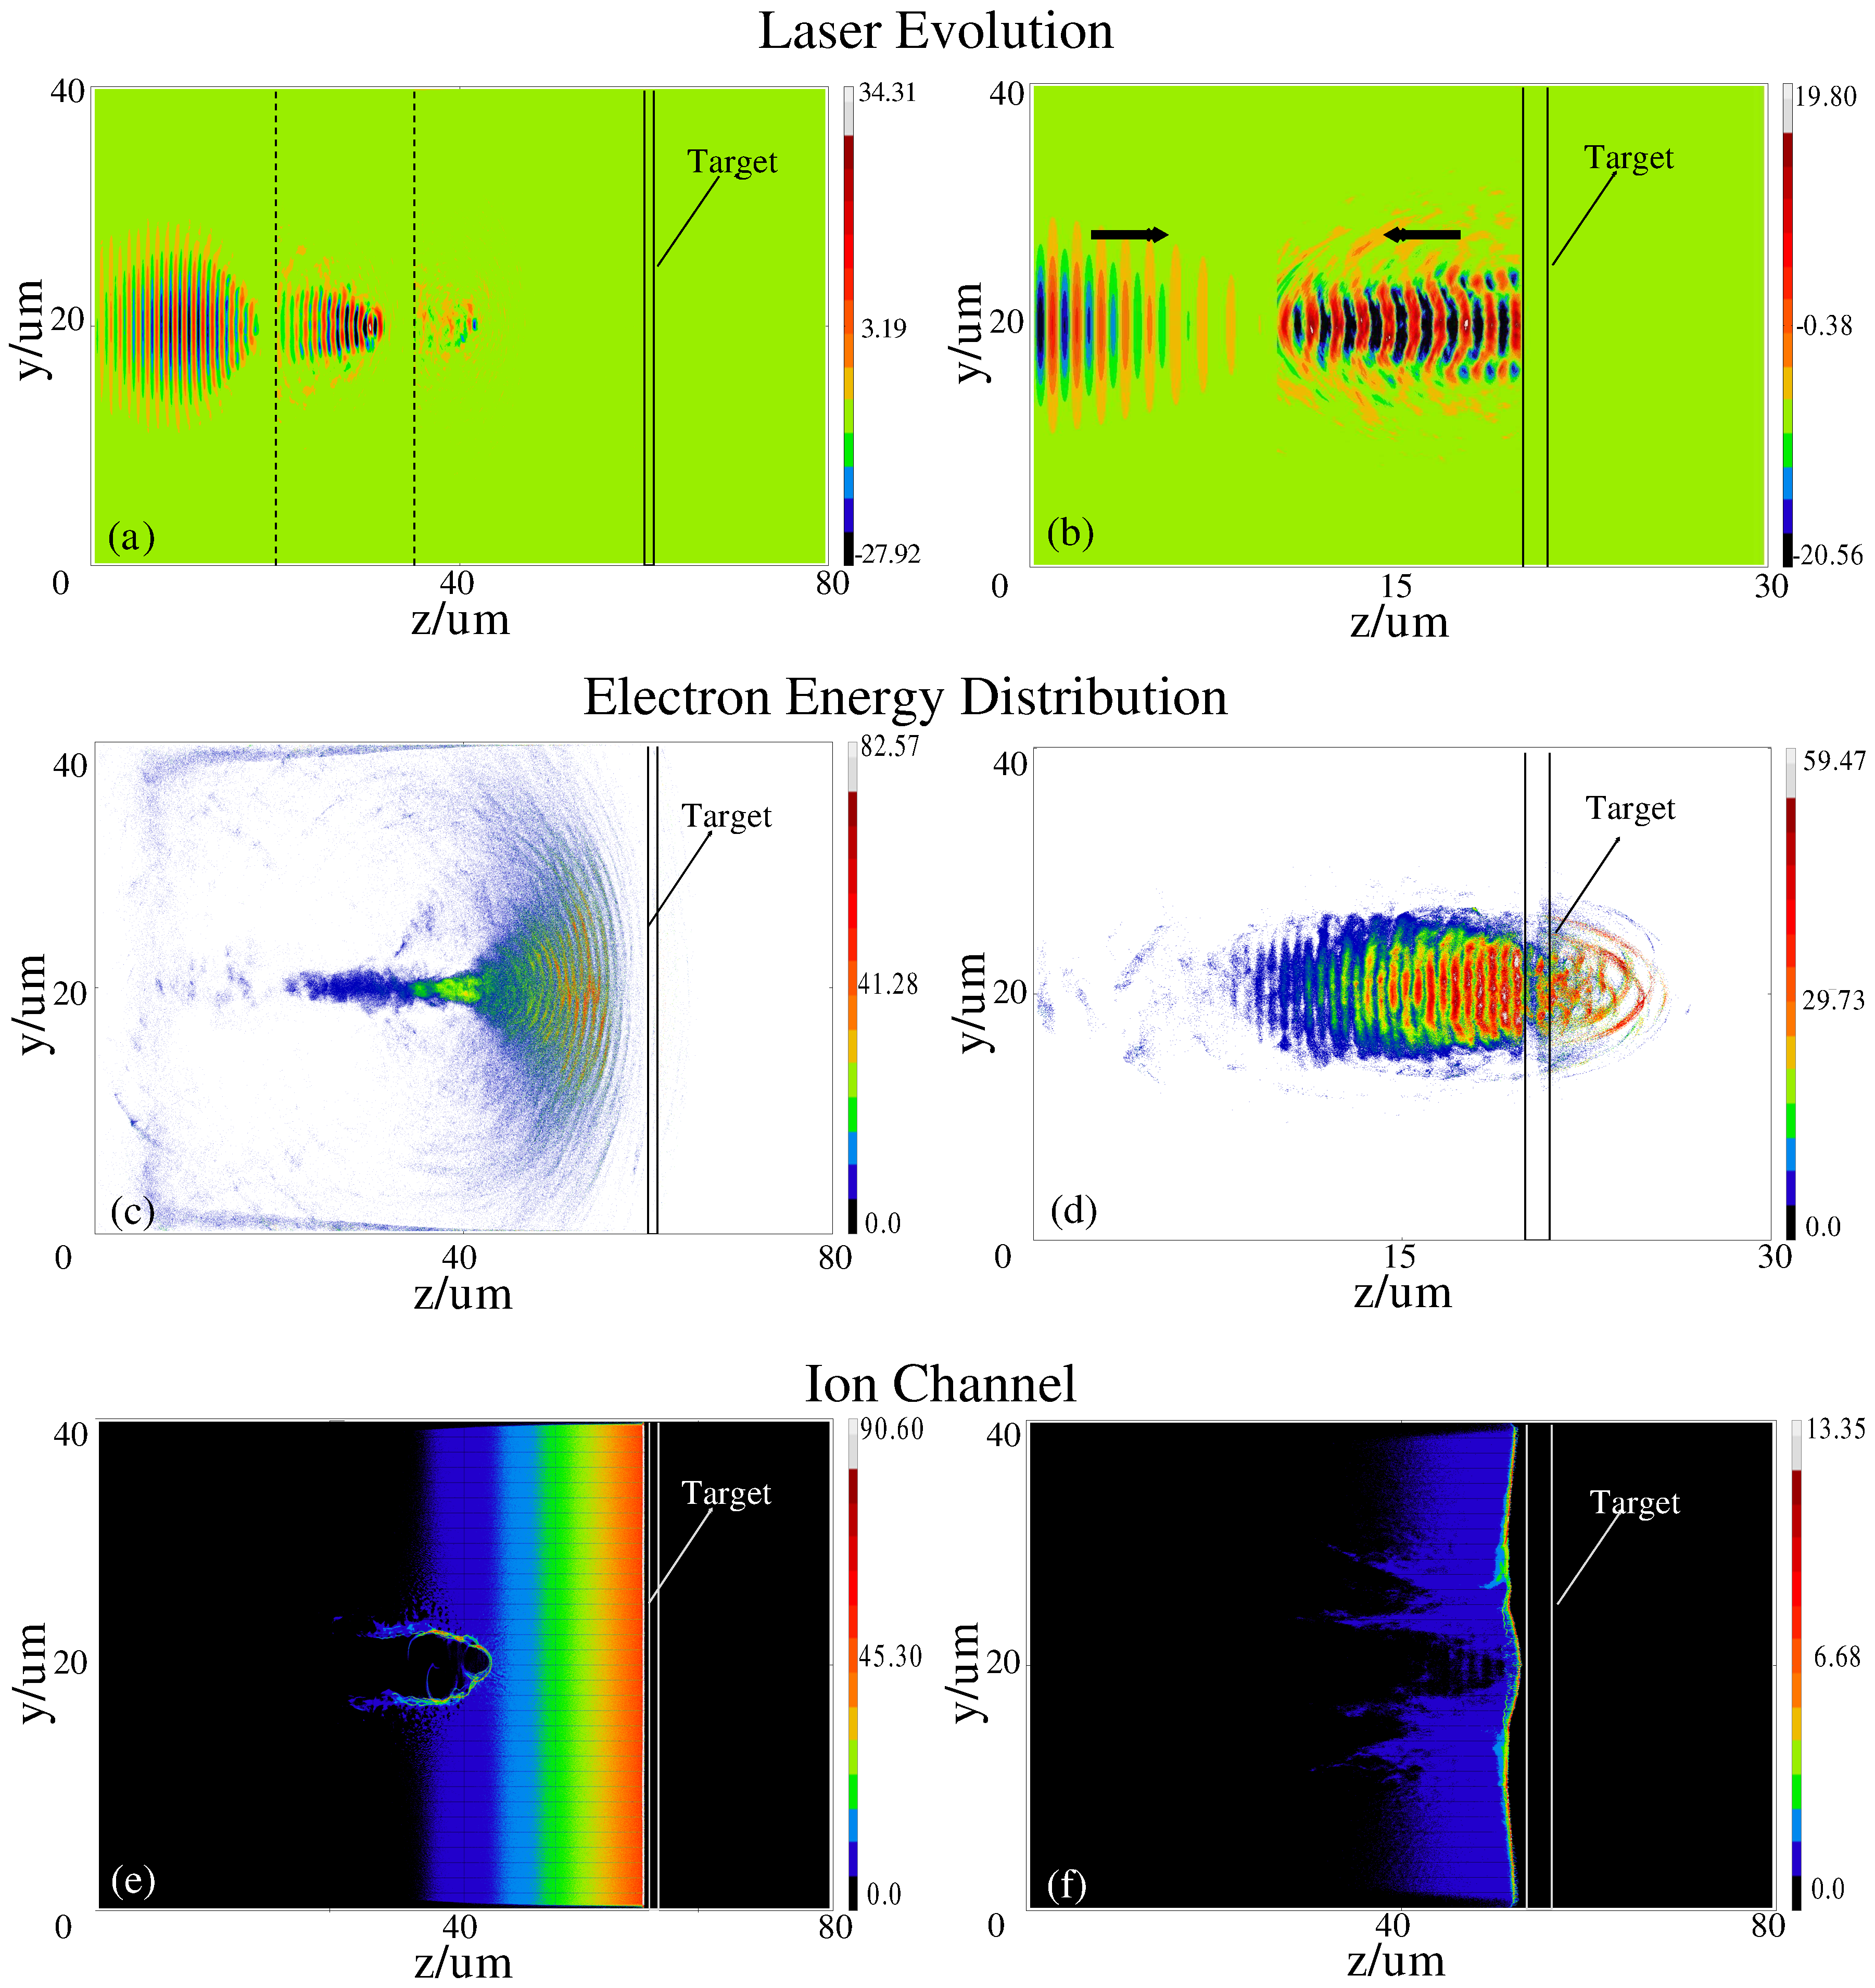
\includegraphics[width=\MyFactor\textwidth]{Img/laserEvolution1.eps}
  \caption{参照组中激光聚焦及共振电子产生和传输}
  \label{fig:laserEvolution1}
\end{figure}


对于以上三种情况,我们考虑了激光能量的吸收并得到了质子能谱,并使用没有预等离子体膨胀的情况进行参照,其结果在\ref{fig:laserAbsorption}(d)。能谱的统计采用了加速过程结束之后质子能量的统计,红色曲线代表‘最优’情况,其能量可以达到$90MeV$,蓝色的‘长脉冲’情况和黑色的‘短脉冲’情况相对较低,分别为$47MeV$,$65MeV$。但是对比绿色的‘无烧蚀’情况,质子能量都有显著提高。同时我们对最优情况,使用mora的自由膨胀的模型进行验证,电子的温度由\ref{eqn:DLAtemperature},而且电子的密度可以从模拟中得到相应的值,加速的时间可估计为$1.3 \tau_{laser}$\cite{fuchs2006laser},带入\ref{eqn:ionMaxenergy}中,得到加速的能量应该在90MeV。


\begin{figure}[!htbp]
  \centering
  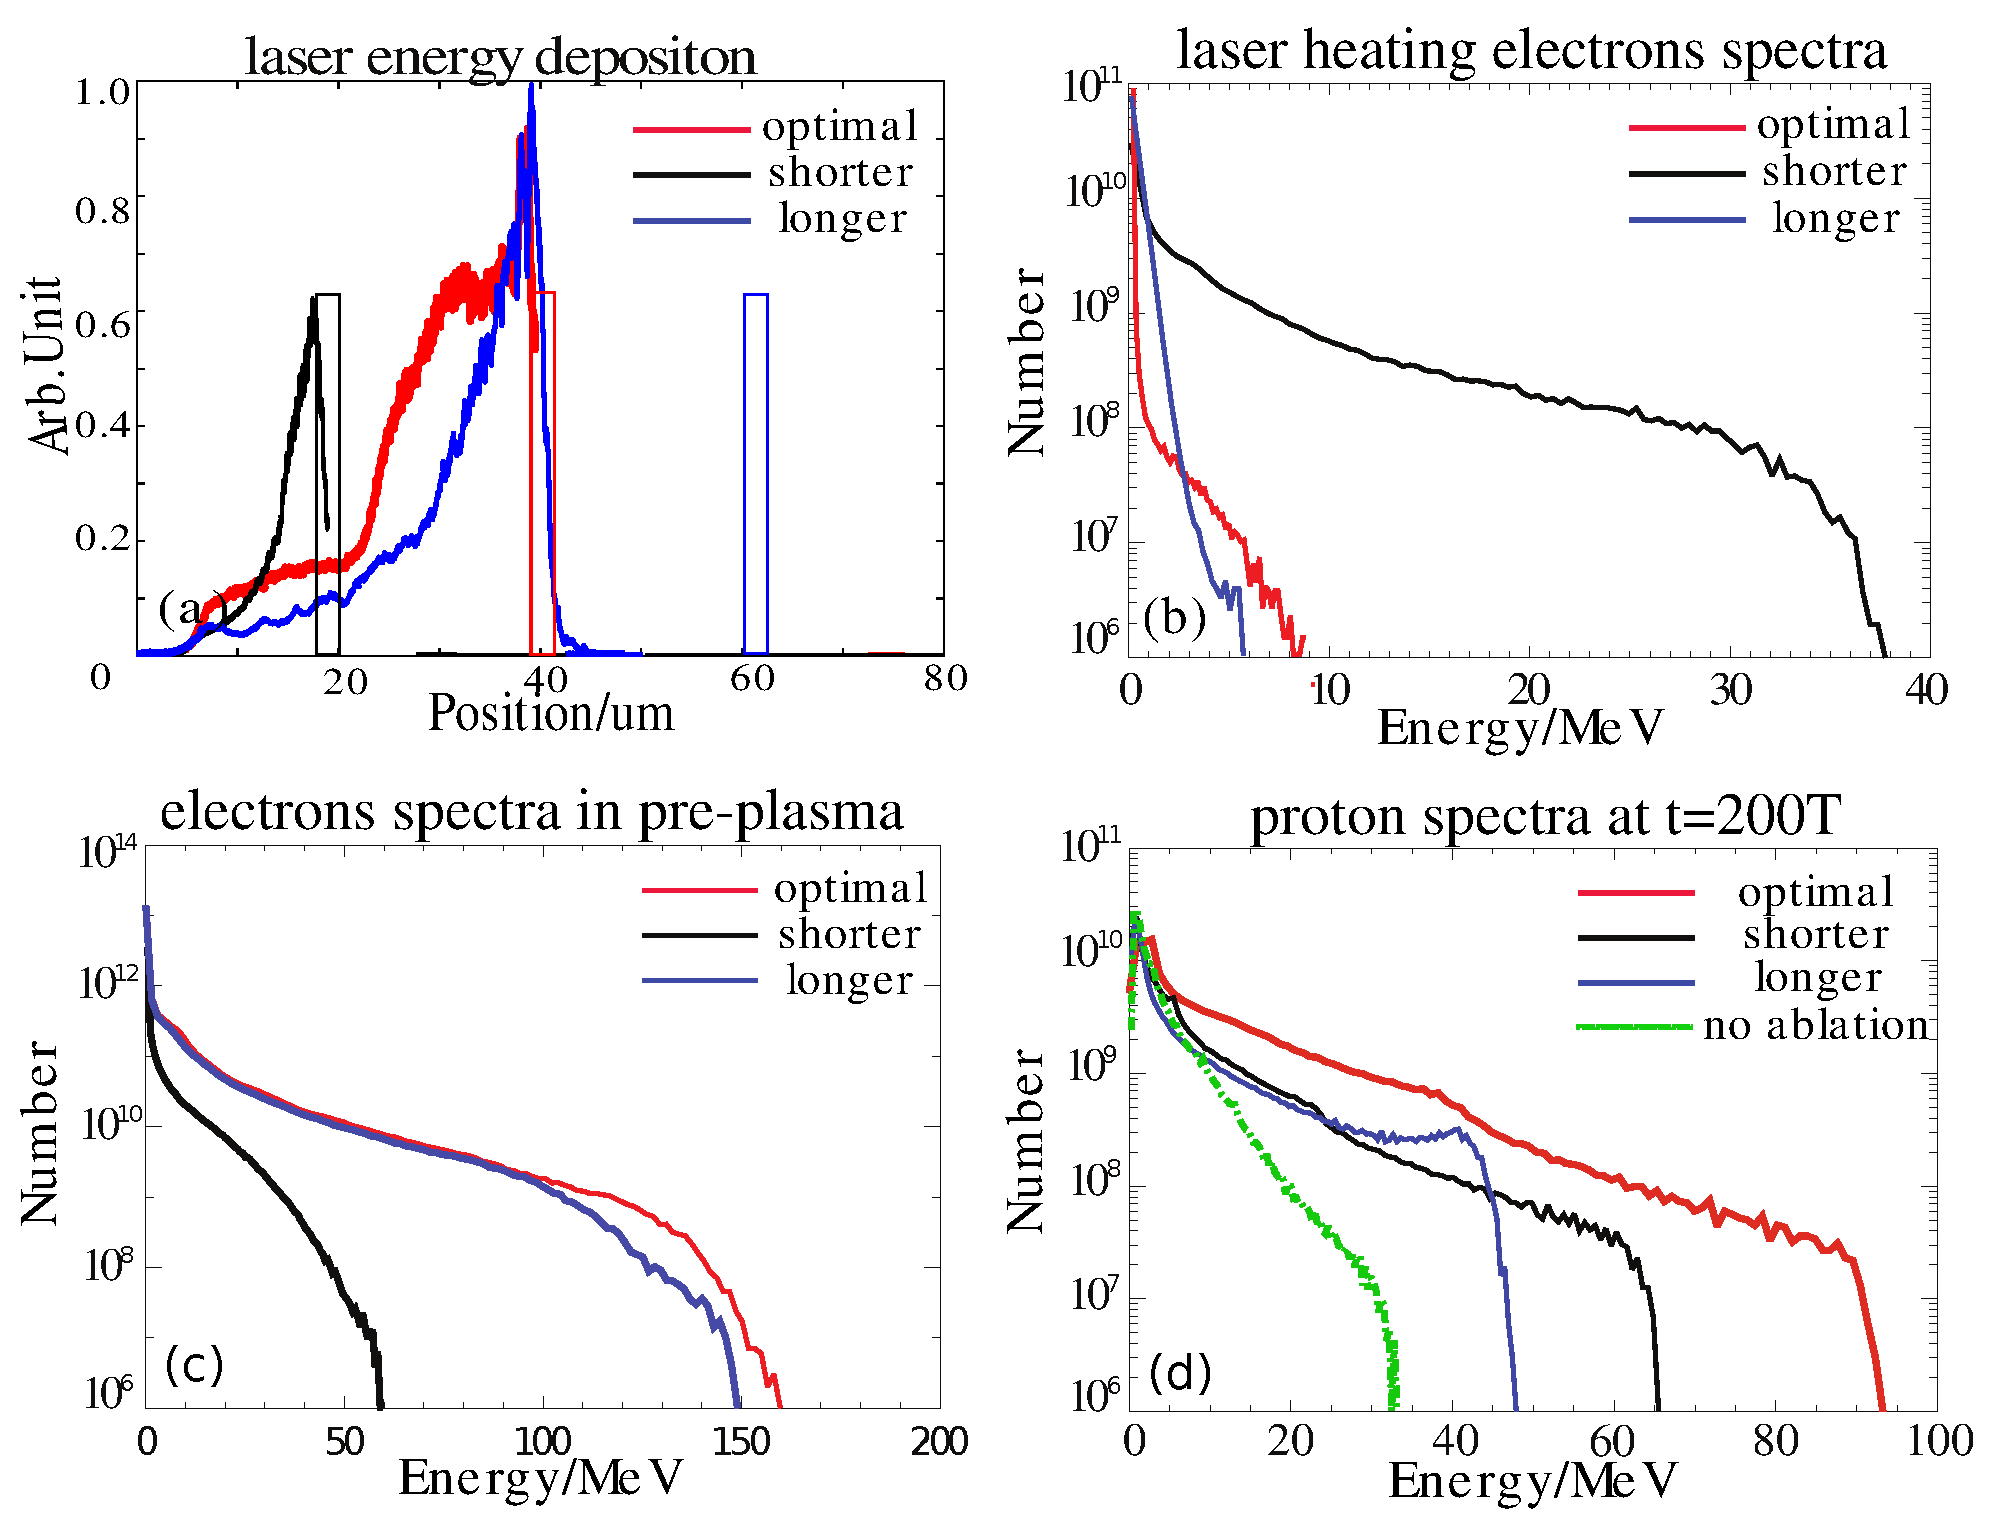
\includegraphics[width=\MyFactor\textwidth]{Img/laserAbsorption.eps}
  \caption{各组中激光能量的吸收}
  \label{fig:laserAbsorption}
\end{figure}



与此可见,由预脉冲产生的预等离子体对于质子加速可以起到增强的作用,而其增强效果存在最优的情况,对应于烧蚀脉冲与激光主脉冲之间的匹配关系。根据\ref{eqn:OptimalCondition},在固定预脉冲与主脉冲的强度的前提下,预脉冲的持续时间应该是和主脉冲的持续时间满足如下关系${\tau}_{abl} \propto  \tau_{cpa}$,呈现一定的正比关系。这就意味着,对于固定预脉冲以及烧蚀脉冲强度的情况,脉冲持续时间在匹配关系时,可以实现最优的增强效果。正如仿真中得到的结果, 脉冲持续时间过短或者过长的预脉冲都减弱了增强效果。在仿真中通过改变预脉冲以及主脉冲参数,得到预脉冲与主脉冲的匹配关系在\ref{fig:scanDuration}。散点是仿真结果,曲线是根据\ref{eqn:OptimalCondition}做出。二者在一定范围内符合,然而在脉冲宽度过大和过小的情况下,偏离了理论分析的结果。其原因在于,一些基本假设不再成立。例如:脉冲持续时间增长之后的能量吸收率不再是一个常量,而是和脉冲参数存在一定的关系;而在脉冲尺寸比较小的时候,由于激光与临界密度等离子体的作用时间不足,未能完全的进行能量转化,\ref{eqn:OptimalCondition}略微过估计了激光的吸收。


\begin{figure}[!htbp]
  \centering
  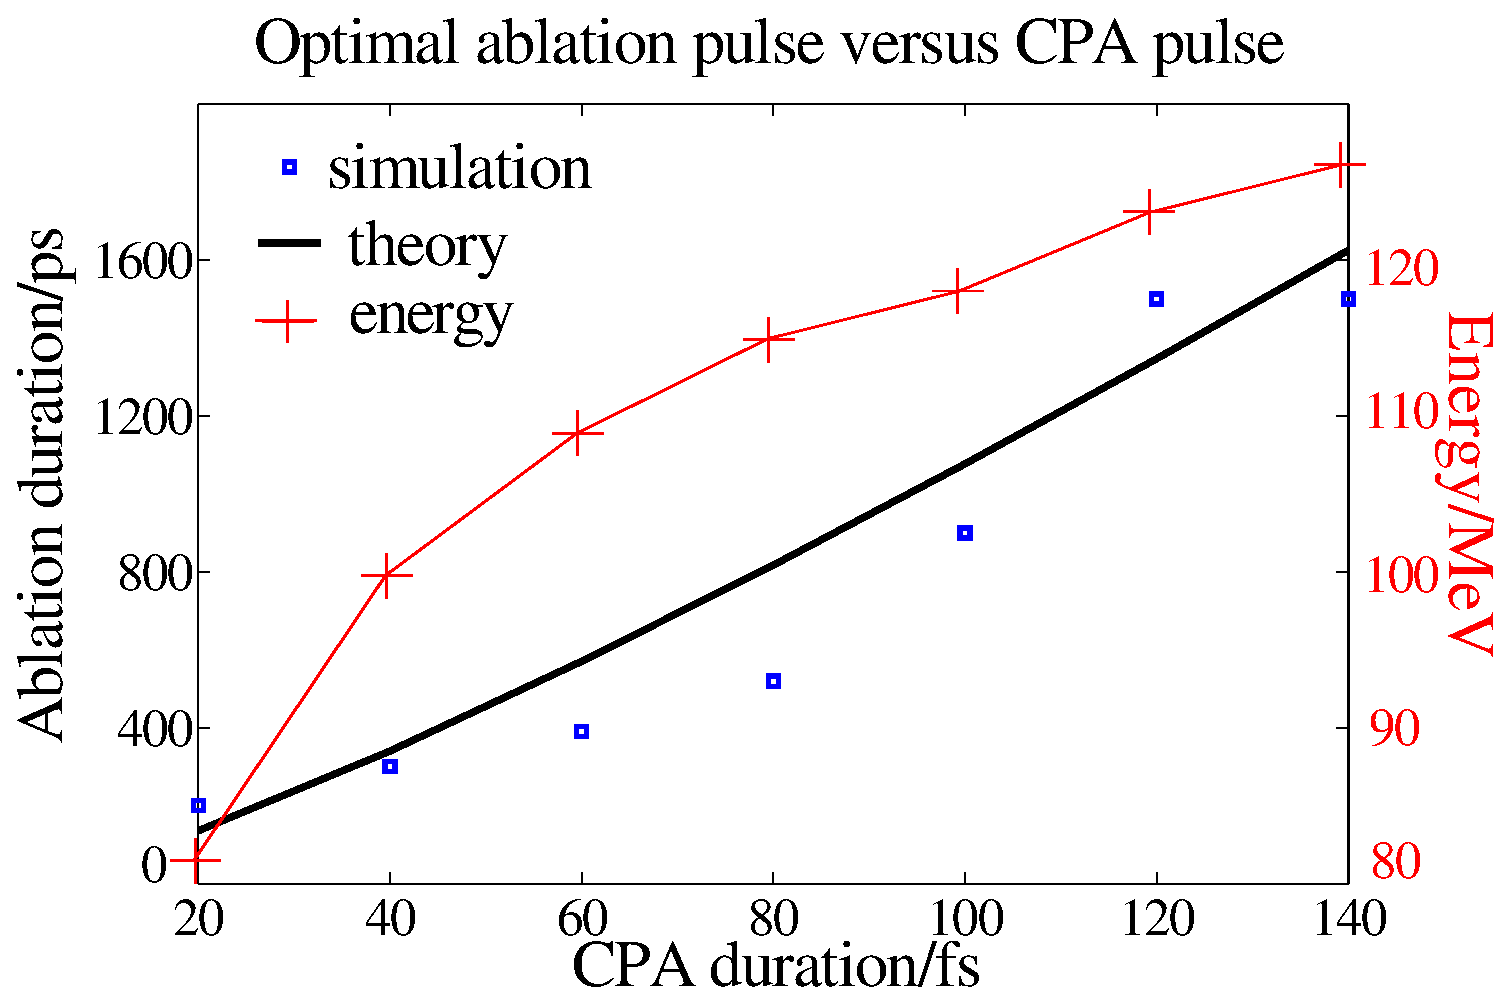
\includegraphics[width=\MyFactor\textwidth]{Img/scanDuration.eps}
  \caption{脉冲持续时间对于加速的影响}
  \label{fig:scanDuration}
\end{figure}



对于实验,我们有相应的实验的验证作为比较,在2008年,macknnea的实验就在一定程度上对于理论分析做出了相应的分析,因为在实验的参数如下,其强度与本文中的模拟的参数是近似的,烧蚀脉冲的持续时间以及主脉冲的持续时间相对较长,但是符合理论推导中的比例关系,因此间接证明了在较长的主脉冲的前提下,最优的加速过程对应于特定的一个激光的持续时间。同时实验中加速粒子的能量远远低于理论的预期的结果,很大原因是由于实验中使用的靶的厚度较大,25微米,这样的厚度下很难保证产生的高品质的共振电子部发生相应的发散,导致最终的及加速效果大打折扣。在实验中的脉冲持续时间是由于烧蚀脉冲的时间来决定的。烧蚀脉冲的时间用于控制激光等离子体的膨胀时间,而时间和膨胀的尺度存在直接的正比的关系,因此存在一定的关系决定最终的关于膨胀的尺度与激光脉冲的匹配关系,这一关系决定了相应的最优加速的过程是由于主脉冲激光和烧蚀脉冲的参数之间存在相应的匹配关系来决定的。一般来说,激光设备的主脉冲很难做出很大的调整,而相应的烧蚀脉冲由于其强度较低,控制的难度也相对较小,可以考虑通过控制烧蚀脉冲的强度以及脉冲持续时间来控制整个的加速的增强的过程。由于最优秀的加速过程往往存在唯一的对应的烧蚀脉冲,这对于实验中的控制是很有好处的,大大提高了相应的可控制的难度。




总的来说,使用预脉冲对于激光离子加速进行增强,是将传统意义上的‘有害’的预脉冲加以利用使其成为促进部分。  这一点对于实验有着一定的指导意义,通过调整烧蚀脉冲以及主脉冲的脉冲持续时间,改变加速离子的能量与束流的发散度,使得激光加速在一定程度上可控。从实验的可行性上,对于激光的控制在实验上更容易实现,对于给定的主脉冲激光,烧蚀激光可以使用激光预脉冲或者另一束独立的激光脉冲。控制其强度以及脉冲持续时间,使其满足最优增强效果,实现加速。




总结,预脉冲以及预等离子体在超强激光与等离子体作用的过程中是不可避免的,在离子加速的过程中,对于加速离子的能量可能起到正面或者反面的作用,直接与等离子体的密度分布有一定的关系,当等离子体的密度分布可以有助于产生共振电子的时候,由于激光的吸收得到有效的增强,进一步的加速的电子的效率得到显著的提升,而在另一方面,如果等离子体的密度的分布无法实现共振电子的条件,而且预脉冲由于强度比较的强,轻易的破坏掉了靶子的后表面结构,那么与等离子体起到的就是一种负面的作用因为无法通过破坏的加速面实现有效的加速电场的形成,在这种条件下的,加速就显得十分的没有意义了。 因此需要对于激光的与脉冲进行相应的控制,而这种控制的核心部分在于对于预脉冲的脉冲时间的控制。 因为时间的控制就决定了相应的预等离子体的分布。而且在给定的激光的强度以及激光的脉冲持续时间的基础上,有最优的预脉冲参数使得激光加速得到的离子的能量达到最高的值,这也是增强效果的最有意义的用途。在这样的基础上我们提出了使用烧蚀脉冲的方法对于传统的激光加速的方法进行相应的改进。烧蚀脉冲的参数考虑了实验室环境下常见的预脉冲的参数,并且对于不同预脉冲脉冲持续时间进行了深入的分析,得到了对于加速有最优效果的加速方案,因为在此基础上的加速,将最大化的实现激光到离子的能量转化。综合考虑实验的可行性,以及加速增强效果,这种方案可以使一种在现有的实验室环境下 的有效的方法,且其操作性强,需要控制的是激光的参数,而不是进行微结构的靶的制作,相应的技术层面的要求更合适目前的实验室的环境的需求。对比于没有烧蚀脉冲的情况,得到的加速的质子的能量提高了响应的3倍以上的量。相信这种技术可以在实验中取得相应的突破,使得激光离子加速的能量步入到百MeV的数量级。此方案的一个优势在于变废为宝,因为在实验中不需要引进 外界的参量,需要的是性能稳定的激光器设备以及分光技术,使得激光的脉冲可以被分成两部分一部分通过放大技术成为主脉冲,另一部分则可以完全用来当做烧蚀脉冲实现对于靶的烧蚀。在这样的设计中,很重要的一点就是主激光以及烧蚀激光之间的匹配关系,因为预脉冲的持续时间决定了相应的预等离子体的分布的情况。在预等离子体中的共振电子的产生是加速增强的直接的原因,没有主激光与预脉冲之间的匹配关系,就很难真的存在对于加速的最优的增强的效果。这是整个章节的核心的地方,也是这种方案的核心,是对于加速在一定程度上进行了相应的控制使得加速的离子的能力可以满足在一定的范围的分布,而且离子的束流的发散程度是和激光的参数相关的,实现了相应的关于控制的要求。



